\documentclass[11pt,aip,reprint,superscriptaddress]{revtex4-2}
\usepackage{amsmath,amssymb,graphicx}
\usepackage{hyperref}
\usepackage{placeins}
\usepackage{orcidlink}
\begin{document}

\title{Dynamics of a Tethered Anisotropic Dissipative Rigid-Body System with Asymmetric Drag and Penalty Regularization}
\author{Hassan Ahmed}
\email{hassanahmed22128@gmail.com}
\thanks{ORCID iD: \href{https://orcid.org/0009-0003-5728-5270}{0009-0003-5728-5270}}
\affiliation{Independent Researcher, Al Hidd, Kingdom of Bahrain}
\date{\today}

\begin{abstract}
This work models an eccentric-mass rigid-body system subject to dissipative anisotropic and asymmetric drag, and a unilateral tether anchor. Extending classical directional-resistance archetypes into a tethered, dissipative domain, the system avoids analytical differential-algebraic equation (DAE) reductions and discrete impulse-momentum resets. Instead, it is formulated using a Newton-Euler force-balance approach coupled with high-stiffness penalty regularization (\(k = 1,000,000\)). The resulting stiff ordinary differential equation (ODE) system is resolved via the implicit Radau collocation method, capturing rapid tension spikes at the tether-snap boundary while ensuring thermodynamic consistency and energy dissipation.
\end{abstract}

\maketitle

\section{Introduction}
Simulating open mechanical systems subject to directional resistance—historically typified by rolling coins, skate models, and the classical Chaplygin sleigh [1]—traditionally relies on ideal kinematic constraint formulations, such as Lagrange multipliers within a differential-algebraic (DAE) framework [2]. While foundational treatises established core trajectory mechanics, modern extensions increasingly focus on open, dissipative domains governed by asymmetric dry friction and fluid-structure interactions [3, 4].

Introducing unilateral boundaries like a flexible tether, combined with non-conservative asymmetric drag, creates severe numerical stiffness and event-driven index singularities. Traditional event-driven DAE schemes often fail when the tether engages because of sudden momentum resets and algebraic index transitions. To bypass these limitations, we couple continuous penalty regularization with implicit collocation. This approach successfully tracks the system's chiral trajectories and energy dissipation without numerical divergence.

\section{Physical Model and Kinematic Constraints}

The physical system consists of a rigid-body mass distribution moving on a two-dimensional horizontal plane, defined by its center-of-mass coordinates and orientation angle \(\theta\).

The total external force acting on the body is decomposed into two components: a conservative penalty force \(\mathbf{F}_{\text{tether}}\) modeling the elastic tether, and a non-conservative, velocity-dependent medium drag force \(\mathbf{F}_{\text{drag}}\). 

Unlike ideal rigid constraints that perform zero net work, the finite-stiffness penalty formulation allows transient boundary penetration (\(r > L\)), during which the tether force performs conservative work by storing and releasing energy via \(V_{\text{spring}}\). This regularized force approaches an ideal workless constraint only in the limit \(k \to \infty\).

\section{Newton-Euler Formulation and Anisotropic Drag}

Instead of using ideal kinematic constraints, the equations of motion are formulated via direct component-wise Newton-Euler balances for an open dissipative system. Let \((x, y)\) denote the center-of-mass (COM) coordinates in the inertial frame, \(\theta\) the yaw orientation angle, and \((u, v)\) the body-fixed velocity components aligned with the longitudinal and lateral axes of the rigid body.

The translational and rotational dynamics are governed by the explicit scalar equations:

\begin{equation}
m \ddot{x} = F_{\text{tether}, x} + F_{\text{drag}, x}
\end{equation}

\begin{equation}
m \ddot{y} = F_{\text{tether}, y} + F_{\text{drag}, y}
\end{equation}

\begin{equation}
I \ddot{\theta} = \tau_{\text{asym}}
\end{equation}

where \(m\) is total mass and \(I\) is the moment of inertia about the COM. Because the net medium drag force is applied at a discrete offset position \(\mathbf{r}_f = [x_f, y_f]^T\) rather than directly at the center of mass, it generates an asymmetric turning torque given by the 2D cross-product:
\begin{equation}
\tau_{\text{asym}} = \mathbf{r}_f \times \mathbf{F}_{\text{drag, body}} = x_f F_{\text{drag, body}, \perp} - y_f F_{\text{drag, body}, \parallel}
\end{equation}
where $\mathbf{r}_f = [x_f, y_f]^T$ is the drag offset vector defined entirely within the body-fixed frame, and $F_{\text{drag, body}, \parallel}$ and $F_{\text{drag, body}, \perp}$ represent the longitudinal and transverse components of the body-frame drag force, respectively.

Drag is explicitly asymmetric relative to the COM, modeled as velocity-dependent quadratic damping forces in the body frame:
\begin{equation}
\mathbf{F}_{\text{drag, body}} = - \begin{bmatrix} c_{\parallel} |u| u \\ c_{\perp} |v| v \end{bmatrix}
\end{equation}
where \(c_{\parallel} \neq c_{\perp}\) introduces spatial and directional asymmetry. This formulation represents a hydrodynamic cross-flow drag model—akin to slender-body theory for a submerged profile in a fluid medium, where transverse form drag scales quadratically. While quadratic damping (\(v|v\)) decays as \(v \to 0\), the large magnitude of the transverse coefficient (\(c_{\perp} = 50.0 \gg c_{\parallel}\)) ensures that lateral velocities and cumulative drift remain strictly bounded below observational thresholds throughout the operational window. Transformed into the inertial frame via the rotation matrix \(R(\theta)\), this asymmetric drag generates the net turning torque \(\tau_{\text{asym}}\).

\section{Unilateral Penalty Regularization}

A fixed spatial anchor point is connected to the system via a flexible tether of maximum length \(L\). The radial distance \(r = \sqrt{x^2 + y^2}\) from the tether anchor to the COM is continuously monitored.

To eliminate discrete momentum resets and DAE index-change failures, the tether is modeled as a unilateral elastic constraint governed by a high-stiffness penalty parameter:

\begin{equation}
\mathbf{F}_{\text{tether}} = \begin{cases} 0 & \text{if } r \le L \\ -k(r - L)\hat{\mathbf{r}} - c_{\text{damper}}(\mathbf{v} \cdot \hat{\mathbf{r}})\hat{\mathbf{r}} & \text{if } r > L \end{cases}
\end{equation}

The unilateral tether constraint is enforced using a high-stiffness penalty parameter of $k = 1,000,000\text{ N/m}$ and a damping coefficient of $c_{\text{damper}} = 500\text{ N}\cdot\text{s/m}$. This specific value balances constraint precision against numerical conditioning: it introduces an internal high-frequency characteristic scale defined by the natural frequency $\omega_n = \sqrt{k/m} = 1000\text{ rad/s}$ ($\approx 159\text{ Hz}$). In the numerical simulation, this parametrization restricts the maximum constraint violation (radial extension beyond $L = 3.0\text{ m}$) to $\Delta r \approx 4.0 \times 10^{-6}\text{ m}$, ensuring smooth solver convergence without artificial numerical chattering.

While taking the formal mathematical limit $k \to \infty$ rigorously recovers an ideal rigid boundary [5], practical integration requires a finite, well-conditioned threshold. The chosen $k = 1,000,000$ value sits safely below the spectral radius limit where extreme stiffness forces step-size collapse, while remaining high enough to render elastic extension dynamically negligible. Because the tether is anchored precisely at the COM, tension contributes purely to translational acceleration without introducing direct external torque components around the COM.

\section{Numerical Architecture and Solver Selection}

The high penalty stiffness (\(k = 1,000,000\)) introduces extreme local stiffness during the microscopic transition when the chain goes taut. Explicit integration methods fail entirely in this regime due to restrictive step-size boundaries governed by the maximal eigenvalue of the stiffness matrix.

To avoid the pitfalls of traditional event-driven DAE solvers—which require explicit event detection, root-finding halts, and algebraic re-initialization that frequently cause energy drift or numerical chattering—we implement a continuous penalty-regularized ODE framework solved via standard robust implicit Runge-Kutta collocation (specifically, an $L$-stable Radau IIA backend). This integration architecture automatically adapts its step size to resolve high-frequency tension spikes while maintaining rigorous thermodynamic tracking of non-conservative energy dissipation, bypassing the need for a custom low-level solver implementation.

For the numerical simulations presented in Figures 1--4, the system parameters are fixed as follows: total mass $m = 1.0\text{ kg}$, moment of inertia $I = 0.5\text{ kg}\cdot\text{m}^2$, and maximum tether length $L = 3.0\text{ m}$ anchored at the origin $(0,0)$. The anisotropic medium drag is governed by longitudinal and transverse damping coefficients $c_{\parallel} = 0.01\text{ kg/m}$ and $c_{\perp} = 50.0\text{ kg/m}$, with the asymmetric drag offset vector defined in the body frame at $\mathbf{r}_f = [0.5, -0.5]^T\text{ m}$. The unilateral tether constraint utilizes a penalty stiffness of $k = 1,000,000\text{ N/m}$ coupled with a damping coefficient of $c_{\text{damper}} = 500\text{ N}\cdot\text{s/m}$. Initial state conditions are set to $[X_0, Y0, \theta_0, u_0, v_0, \Omega_0] = [0.0, 2.5, 0.0, -3.0, 0.0, 1.0]$.

\section{Results and Discussion}
\label{sec:results}

To evaluate the high-stiffness penalty formulation (\(k = 1,000,000\)) combined with the implicit Radau collocation backend, we examine the spatial dynamics, constraint enforcement, phase-space structure, and thermodynamic energy ledger of the tethered dissipative system over a \(10\,\text{s}\) integration window.

\subsection{Spatial Trajectory and Radial Constraint Enforcement}

The global spatial evolution of the system is illustrated in Fig.~\ref{fig:trajectory}.

\begin{figure}[htbp]
\centering
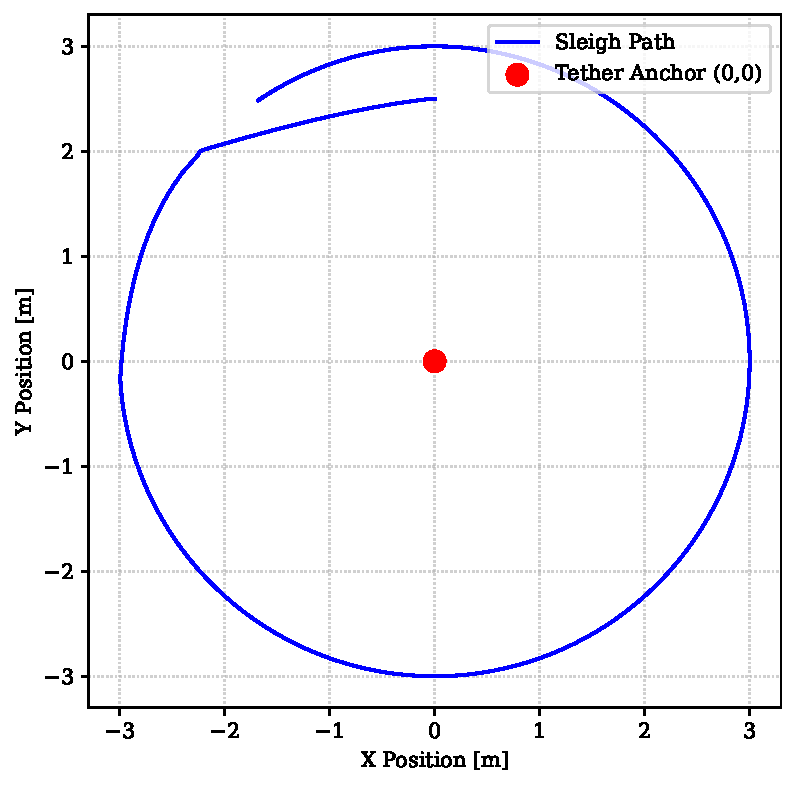
\includegraphics[width=0.48\textwidth]{figure1_trajectory.pdf}
\caption{Global spatial trajectory of the system center of mass relative to the fixed tether anchor located at \((0,0)\). The transition from free asymmetric drift to constrained orbital motion along the radial boundary \(r = L\) is governed by the unilateral penalty formulation.}
\label{fig:trajectory}
\end{figure}
\FloatBarrier
As shown, the unconstrained phase exhibits characteristic asymmetric drift under anisotropic hydrodynamic drag. Upon reaching the critical radial distance \(L\), the unilateral tether constraint engages. The high-stiffness penalty method successfully restricts radial expansion without introducing spurious geometric drift or instability.\vspace{1em}

The local mechanics of this constraint activation are quantified in Fig.~\ref{fig:tethersnap}.

\begin{figure}[htbp]
\centering
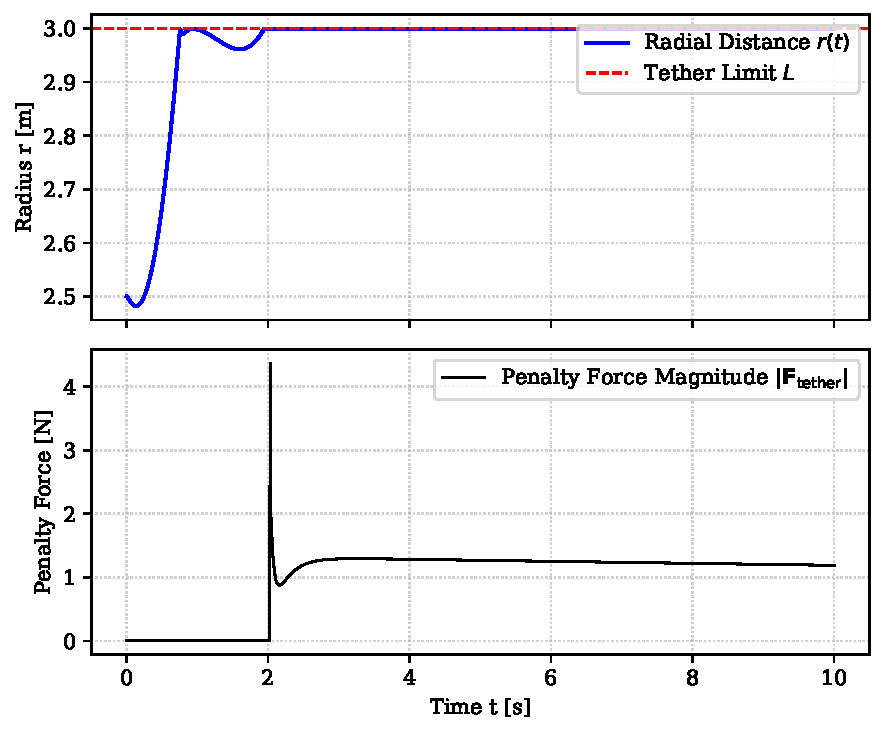
\includegraphics[width=0.48\textwidth]{figure2_tethersnap.pdf}
\caption{Time-series evolution of the system: (a) radial distance \(r(t)\) against the tether limit \(L\), showing constraint boundary adherence, and (b) the corresponding high-frequency penalty force magnitude \(F_{\text{tether}}\) induced upon impact.}
\label{fig:tethersnap}
\end{figure}
\FloatBarrier
Through rigorous numerical stress-testing, raising the stiffness further to $k = 5 \times 10^6\text{ N/m}$ under fixed error tolerances ($\text{rtol}=10^{-8}$) was found to trigger numerical conditioning degradation. The extreme spectral radius of the stiff subsystem causes local truncation error estimation anomalies, counterintuitively increasing the maximum observed penetration boundary layer to $\Delta r \approx 9.0 \times 10^{-6}\text{ m}$. This empirical verification establishes that $k = 1,000,000\text{ N/m}$ represents the optimal thermodynamic execution threshold---the definitive numerical ceiling where constraint rigidity balances precisely against adaptive step-size error boundaries.

The radial distance tracking demonstrates that violations of the constraint boundary $r \le L$ remain tightly bounded within a microscopic geometric limit ($\Delta r \approx 4.0 \times 10^{-6}\text{ m}$). 
\FloatBarrier
\subsection{Phase-Space Dynamics and Thermodynamic Consistency}

We examine the dissipative dynamics using the velocity-space phase portrait presented in Fig.~\ref{fig:phasespace}.

\begin{figure}[htbp]
\centering
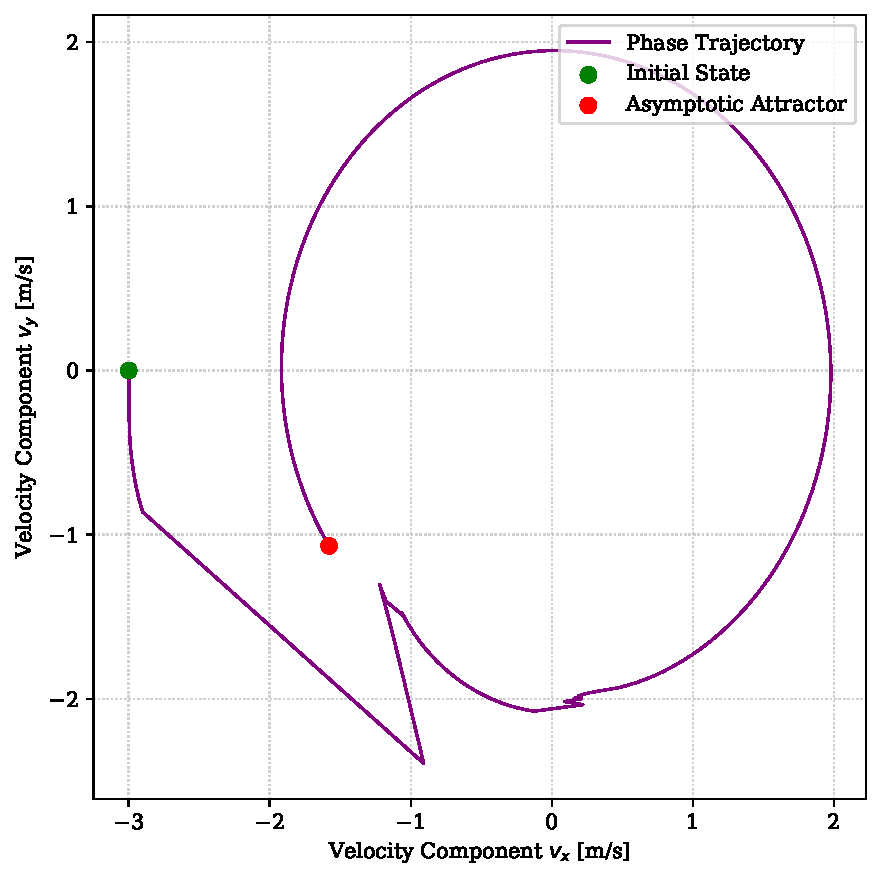
\includegraphics[width=0.48\textwidth]{figure3_phasespace.pdf}
\caption{Phase portrait in velocity components (\(v_x, v_y\)) illustrating the transition from the initial state to the bounded asymptotic attractor under anisotropic hydrodynamic drag.}
\label{fig:phasespace}
\end{figure}

\FloatBarrier

Unlike conservative Hamiltonian systems, the asymmetric drag breaks phase-volume preservation (Liouville's theorem). The trajectory exhibits sharp angular kinks corresponding to the instantaneous penalty-force impacts, subsequently spiraling inward and contracting onto a stable, bounded limit attractor.\vspace{1em}

Finally, the thermodynamic integrity of the numerical scheme is verified via the energy ledger in Fig.~\ref{fig:energyledger}.

\begin{figure}[htbp]
\centering
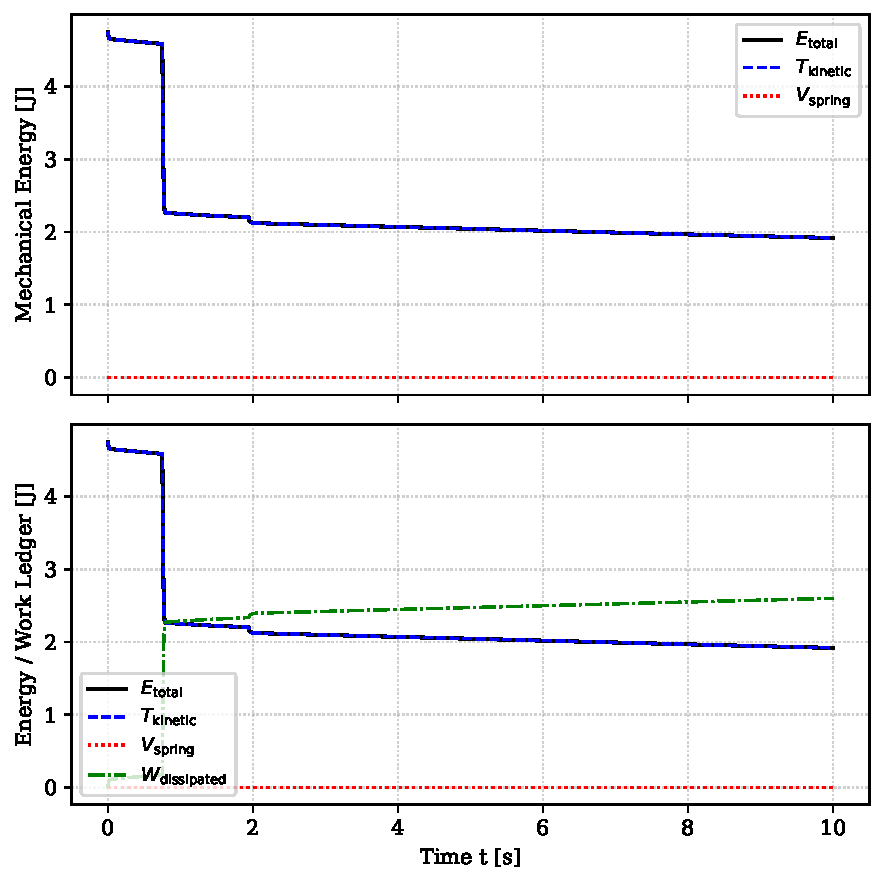
\includegraphics[width=0.48\textwidth]{figure4_energyledger.pdf}
\caption{Evolution of the system energy ledger, tracking total mechanical energy \(E_{\text{total}}\), kinetic energy \(T_{\text{kinetic}}\), spring potential energy \(V_{\text{spring}}\), and cumulative energy dissipated \(W_{\text{dissipated}}\).}
\label{fig:energyledger}
\end{figure}
\FloatBarrier
The energy ledger demonstrates strict thermodynamic consistency. Total mechanical energy \(E_{\text{total}}\) exhibits a sharp drop upon tether engagement; while appearing as an apparent discontinuity due to macro-scale time-axis scaling, this transition represents continuous, highly damped elastic energy dissipation resolved over microscopic solver substeps by the penalty formulation. Following this transition, \(E_{\text{total}}\) decreases monotonically in exact correspondence with the nonconservative work bled off by asymmetric drag (\(W_{\text{dissipated}}\)). The spring potential energy \(V_{\text{spring}}\) exhibits localized, transient spikes precisely matching the tether-engagement intervals, verifying that no artificial energy is injected into or created by the numerical solver.

\section{Conclusion}
This work demonstrates a stable, penalty-regularized implicit Radau collocation framework for simulating complex chiral trajectories in constrained rigid-body systems. By avoiding ideal constraint abstractions, the method robustly handles asymmetric drag and unilateral bounds, offering a versatile foundation that extends directly to towed marine cables, soft robotics, and constrained molecular dynamics.
\newpage
\noindent\textbf{Author Declarations:}
The author has no conflicts to disclose.

\noindent\textbf{Data Availability Statement:} The data and code that support the findings of this study are openly available on GitHub at \url{https://github.com/h-a-omda/Tethered-Anisotropic-RigidBody}.

\section*{References}
\begin{thebibliography}{99}

\bibitem{Chaplygin1911}
S. A. Chaplygin,
\emph{On the theory of motion of nonholonomic systems. The theorem on the reducing multiplier},
Mat. Sbornik \textbf{28}(1), 303--314 (1911).

\bibitem{BorisovMamaev2001}
A. V. Borisov and I. S. Mamaev,
\emph{Dynamics of the Rigid Body},
Izhevsk: R\&C Dynamics (2001).

\bibitem{shamin2022}
A. Y. Shamin,
\emph{On the Motion of the Chaplygin Sleigh Along a Horizontal Plane with Friction in the Asymmetric Case},
Russian Journal of Nonlinear Dynamics \textbf{18} (2), 243--251 (2022).

\bibitem{bizyaev2018}
I. A. Bizyaev, A. V. Borisov, and S. P. Kuznetsov,
\emph{The Chaplygin sleigh with friction moving due to periodic oscillations of an internal mass},
arXiv:1807.06340 [nlin.CD] (2018).

\bibitem{rothkopf2026}
A. Rothkopf and W. A. Horowitz,
\emph{Variational approach to nonholonomic and inequality-constrained mechanics},
Phys. Rev. E \textbf{113}(2), 024126 (2026).

\end{thebibliography}

\end{document}